\documentclass{ctexart}
\usepackage{amsmath, mathrsfs, amsfonts}
\usepackage{tikz}
\usepackage{graphicx}


% library

\begin{document}

\begin{figure}[htp]
    \centering
    \begin{tikzpicture}[>=latex]
        \node (s1) at (0,0) [rectangle, draw=blue!50, fill=blue!20] {均方收敛};
        \node (s2) at (4,0) [rectangle, draw=blue!50, fill=blue!20] {以概率1收敛};
        \node (s3) at (2,-2) [rectangle, draw=blue!50, fill=blue!20] {依概率收敛};
        \node (s4) at (2,-4) [rectangle, draw=blue!50, fill=blue!20] {依分布收敛};
        \draw[->] (s1)--(s3);
        \draw[->] (s2)--(s3);
        \draw[->] (s3)--(s4);

    \end{tikzpicture}

    \caption{<caption>}
\end{figure}


\begin{figure}[htp]
    \centering
    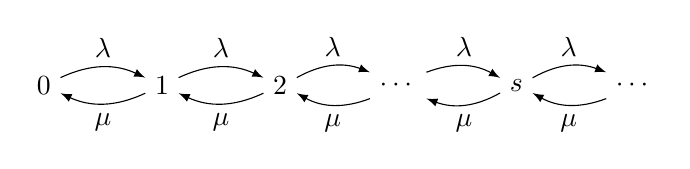
\begin{tikzpicture}[>=latex,scale=1.5]
        \foreach \x/\xtext in {0/0,1/1,2/2,3/\cdots,4/s,5/\cdots}
        {
            \node (s\x) at (\x,0) {$\xtext$};
        }
        \draw[->] (s0) to [bend left=25] node[above]{$\lambda$} (s1);
        \draw[->] (s1) to [bend left=25] node[above]{$\lambda$} (s2);
        \draw[->] (s2) to [bend left=25] node[above]{$\lambda$} (s3);
        \draw[->] (s3) to [bend left=25] node[above]{$\lambda$} (s4);
        \draw[->] (s4) to [bend left=25] node[above]{$\lambda$} (s5);
        
        \draw[<-] (s0) to [bend right=25] node[below]{$\mu$} (s1);    % [bend right=25]==[bend left=-25]
        \draw[<-] (s1) to [bend right=25] node[below]{$\mu$} (s2);
        \draw[<-] (s2) to [bend right=25] node[below]{$\mu$} (s3);
        \draw[<-] (s3) to [bend right=25] node[below]{$\mu$} (s4);
        \draw[<-] (s4) to [bend right=25] node[below]{$\mu$} (s5);


    \end{tikzpicture}

    \caption{<caption>}
\end{figure}

\end{document}